\chapter{Introduction}
\graphicspath{{./introduction/graphs/}}

\onehalfspacing
%======================================================================
\section{Polymer}

Polymers are large molecules that consist of repeating units, called monomers. The number of monomers that a polymer contains is defined as its degree of polymerization, $N$. Thus the molecular weight of a polymer is $M = NM_{mon}$, where $M_{mon}$ is the molecular weight of a monomer. Typically, the backbone of a polymer is composed of carbon atoms connected to each other by covalent bonds. Polymers that contain only one type of monomers are called homopolymers, while those containing more than one type are called heteropolymers \cite{Rubinstein2003}. 

Polymer samples normally exist as a collection of polymer molecules with unequal molecular weights, hence the average molecular weight of the entire sample is described as either number average molecular weight, $M_{n}$, or weight average molecular weight, $M_{w}$: 

\begin{equation}
\label{Mn}
M_{n} = \dfrac{\sum N_{i}M_{i}}{N_{i}}
\end{equation}

\begin{equation}
\label{Mw}
M_{w} = \dfrac{\sum N_{i}M_{i}^{2}}{N_{i}M_{i}}
\end{equation}

where $M_{i}$ is the molecular weight of a polymer chain, and $N_{i}$ is the number of polymer chains with molecular weight $M_{i}$. On both sides of $M_{n}$, there are equal numbers of polymers, while on both sides of $M_{w}$, there are equal weights of polymers. 

Polydispersity index is defined by the ratio of $M_{w}$ to $M_{n}$, and it describes how broad the distribution of molecular weight is. If all the polymers have the same molecular weight, PDI is equal to 1, and the sample is called monodisperse. The larger the PDI is, the broader the molecular weight distribution is, which is normally undesirable. For an intuitive sense of PDI, here is an example. A sample contains half, by number, of polymers with molecular weight 1000, and the other half with molecular weight 2000. $M_{n}$ of this sample is calculated to be 1500, and $M_{w}$ is 1667. Thus PDI of this sample is 1.11, which appears decent, but the corresponding sample is far from pure. In real cases the polymers are more likely to have a Gaussian distribution of different molecular weights rather than shown in this particular example, but this calculation gives us an idea of how PDI could be hiding the actual composition of a polymer sample.

\section{Polymerization}

Synthesized polymers contain a distribution of different molecular weights. Even the most monodisperse synthetic polymers have a polydispersity index (PDI) of about 1.01 \cite{Thakur2016}, which still contain many different $N$ values. This fact is closely related to the process of producing synthetic polymers, polymerization.

Polymerization is the process of connecting monomers together onto a polymer chain. This process could be achieved through different methods. Common methods include step-growth polymerization, chain-growth polymerization, and living anionic polymerization, which is a special case of chain-growth. 

Step-growth polymerization refers to the process in which stepwise reactions among functional groups of monomers form polymers. Typical polymers produced by step-growth include polyamide (nylon), polyester, and polyether \cite{Carraher2003a}. Chain-growth polymerization refers to the process in which unsaturated monomers are added onto the active sites of a growing polymer successively. Typical polymers produced by chain-growth include polyethylene, polypropylene, and polyvinyl chloride \cite{YOUNG2017}. Being a special case of chain-growth, living polymerization is a process in which the termination step of the polymer growth is eliminated, and the rate of chain initiation is much larger than chain propagation, making the polymer growth easier to control. Living anionic polymerization, with anionic propagating species, is one of the most common methods of living polymerization \cite{Halasa1981}. 

Based on different mechanisms, these methods lead to different polydispersity indices. The typical PDI that step-growth leads to is around 2, and for common chain-growth such as free radical polymerization, it is 1.2 $\sim$ 1.5. Living anionic polymerization normally leads to a PDI less than 1.2, which could even reach a number very close to 1, provided with proper conditions \cite{Dotson1995}.

\section{Poly(Ethylene Oxide)}

Poly(Ethylene Oxide), also known as Poly(Ethylene Glycol) or Poly(OxyEthylene), is a polymer with the repeating unit:

\begin{center}
\def\setpolymerdelim#1#2{%
	\def\delimleft{#1}%
	\def\delimright{#2}%
}

\def\makebraces[#1,#2]#3#4#5{%
	\edef\delimhalfdim{\the\dimexpr(#1+#2)/2}%
	\edef\delimvshift{\the\dimexpr(#1-#2)/2}%
	\chemmove{%
		\node[at=(#4),yshift=(\delimvshift)]%
		{$\expandafter\left\delimleft\vrule height \delimhalfdim depth \delimhalfdim width 0pt\right.$};%
		\node[at=(#5),yshift=(\delimvshift)]%
		{$\left.\vrule height \delimhalfdim depth \delimhalfdim width 0pt \expandafter\right\delimright_{\rlap{#3}}$};%
	}%
}

\setpolymerdelim()

\chemfig{\vphantom{CH_2}-[@{op,.75}]CH_2-CH_2-O-[@{cl,0.25}]}
\makebraces[5pt,5pt]{\!\!n}{op}{cl}
\end{center}

PEO has various architectures, including linear, branched, star and comb, and the most widely used type in industry, especially for high molecular weights, is linear PEO. It is soluble in water, acetone, alcohols, benzene, dichloromethane, chloroform, ethanol, methanol, etc., depending on its molecular weight \cite{Brady2017}. 

Low molecular weight PEO (normally below 400 $g/mol$) is liquid at room temperature, and its melting point increases with molecular weight, with an upper limit of \SI{68.9}{\celsius} \cite{Buckley1975}, which is the predicted melting temperature of PEO in the limit of infinite molecular weight.

PEO based materials have advantages over other materials such as non-toxicity, low cost, and electrochemical stability \cite{Xue2015}. Therefore they have a wide range of applications in fields including biology, chemistry, and medicine. Because of its excellent ion conductivity, one of the most promising applications is to act as electrolyte material in lithium ion batteries \cite{Croce1998}. However, it is the amorphous phase in PEO that contributes to ion conductivity, while the linear structure of PEO leads to high crystallinity, which restrains ion transportation especially at low temperatures. Thus, research on PEO crystallization is of great importance.

In this research, the PEO sample purchased from Sigma Aldrich, Inc. has an average $M_{n}$ of 600, which appears as waxy solid at room temperature, and the polydispersity index is not specified in the product information. It has the following chemical structure, with both ends being hydroxy group.

\begin{figure}[H]
	\center
	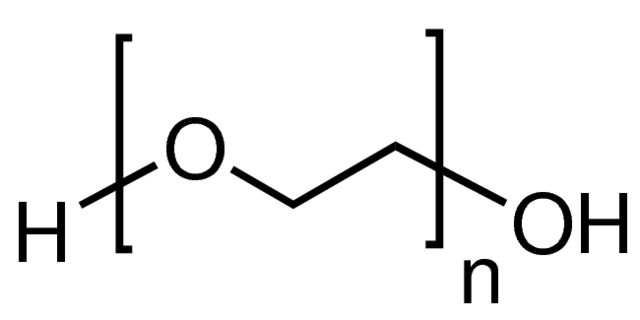
\includegraphics[width=0.3\linewidth]{PEO600}
	\caption[Chemical structure of PEO sample with average $M_{n}$ of 600.]{Chemical structure of PEO sample with average $M_{n}$ of 600. Figure source: "Poly(ethylene glycol) average Mn 600, waxy solid (moist)" from Sigma-Aldrich, 2018 \cite{Sigma-Aldrich2018}.}
	\label{fig:PEO600}
\end{figure}

\section{Importance of $N$}

The degree of polymerization N has an important effect on many properties of polymers. According to Flory-Huggins equation \cite{Rubinstein2003}: 

\begin{equation}
\label{eqn_free energy}
\Delta F_{mix} = kT [\dfrac{\phi}{N} \ln \phi + (1 - \phi) \ln (1 - \phi) + \chi \phi (1 - \phi)]
\end{equation}

\noindent
where the free energy of mixing a polymer with a solvent, $\Delta F_{mix}$, is dependent on $N$. Therefore different $N$'s cause different solubilities. 

Another property that $N$ influences is glass transition temperature $T_{g}$. Glass transition is one of the most crucial phase transitions in polymer science, which refers to the temperature at which the free volume available for molecular motions achieves a minimum. According to Flory-Fox equation \cite{Fox1950a}:

\begin{equation}
\label{eqn_fox-flory}
T_{g} = T_{g,\infty} - \dfrac{K}{M_{n}}
\end{equation}

\noindent
$T_{g}$ is dependent on $M_{n}$, which is directly determined by $N$.

Polymer crystallization is also affected by $N$. One example is atactic polystyrene (aPS). Atactic indicates that the phenyl groups are randomly oriented along the chain. Therefore, crystallization is less preferred for aPS, and thus it has been described as a non-crystal. However, using atomic force microscope (AFM), Yu Chai \textit{et al} \cite{Chai2016} discovered that aPS with $M_{w}$ 600 $g/mol$, which corresponds to a very low $N$, does crystallize. This indicates that $N$ has significant effects on polymer crystallization. One of the many effects of $N$ values on polymer crystallization is related to the end groups. End groups normally contribute to amorphous regions in polymer crystals, and they influence crystal formation process. With different $N$ values, the fractions of end groups are different, which changes the extent of their effect. Therefore, to fully explore the effect of $N$, polymer fractions with different $N$ values must be isolated first.

\section{Polymer crystallization}

Crystallization of large molecules has long been a research topic intensively studied, yet with numerous questions unsolved and mechanisms to be understood. The main factor that causes the essential difference in polymer crystallization and crystallization of a regular small molecule is the long chain nature of a polymer, which results in very different kinetic mechanisms than small molecules. Long chains could easily get entangled, which prevent themselves from being aligned in order in the crystalline lattice. However, crystallization is still possible in certain polymers, often with a much different structure than regular crystals.

In this thesis, PEO is our subject of crystallization study. This linear polymer has many properties in common with n-alkanes, therefore studies on n-alkanes crystallization could also give us insights on our research. For n-alkanes crystallization from melt, investigations have been focused on aspects including crystal structure, chain conformations, nucleation and growth mechanisms, etc. Conformation of n-alkane chains in the crystal include both extended chains and folding of chains \cite{Organ1996,Alamo1993}, where the number of folds depend on chain lengths, crystallization conditions, etc. Nulceation and growth rates of n-alkanes crystals have also been investigated, and most studies are based on experimental methods including X-ray diffraction (XRD), small angle X-ray spectroscopy (SAXS), infrared spectroscopy, optical microscopy, and electron microscopy, as well as computer simulation methods such as molecular dynamics (MD) simulations \cite{Anwar2013,Yamamoto2016}.

In Chapter \ref{chap_analysis}, a more detailed review on polymer crystallization and PEO crystallizaiton in particular is provided, mainly focusing on the thermodynamics and crystal structure. In Chapter \ref{chap_growth}, polymer crystallization kinetics, including nucleation and crystal growth mechanisms are reviewed.
